\section{Resultados y discusión}

\subsection{Análisis bibliométrico y mapeo de palabras clave}

Para establecer la estructura conceptual e identificar los frentes de
investigación principales, se realizó un análisis bibliométrico de los 42
documentos seleccionados. Mediante el uso de VOSviewer, se generó un mapa de
coocurrencia de palabras clave para delimitar el panorama temático.

\begin{figure}[htbp]
	\centering
	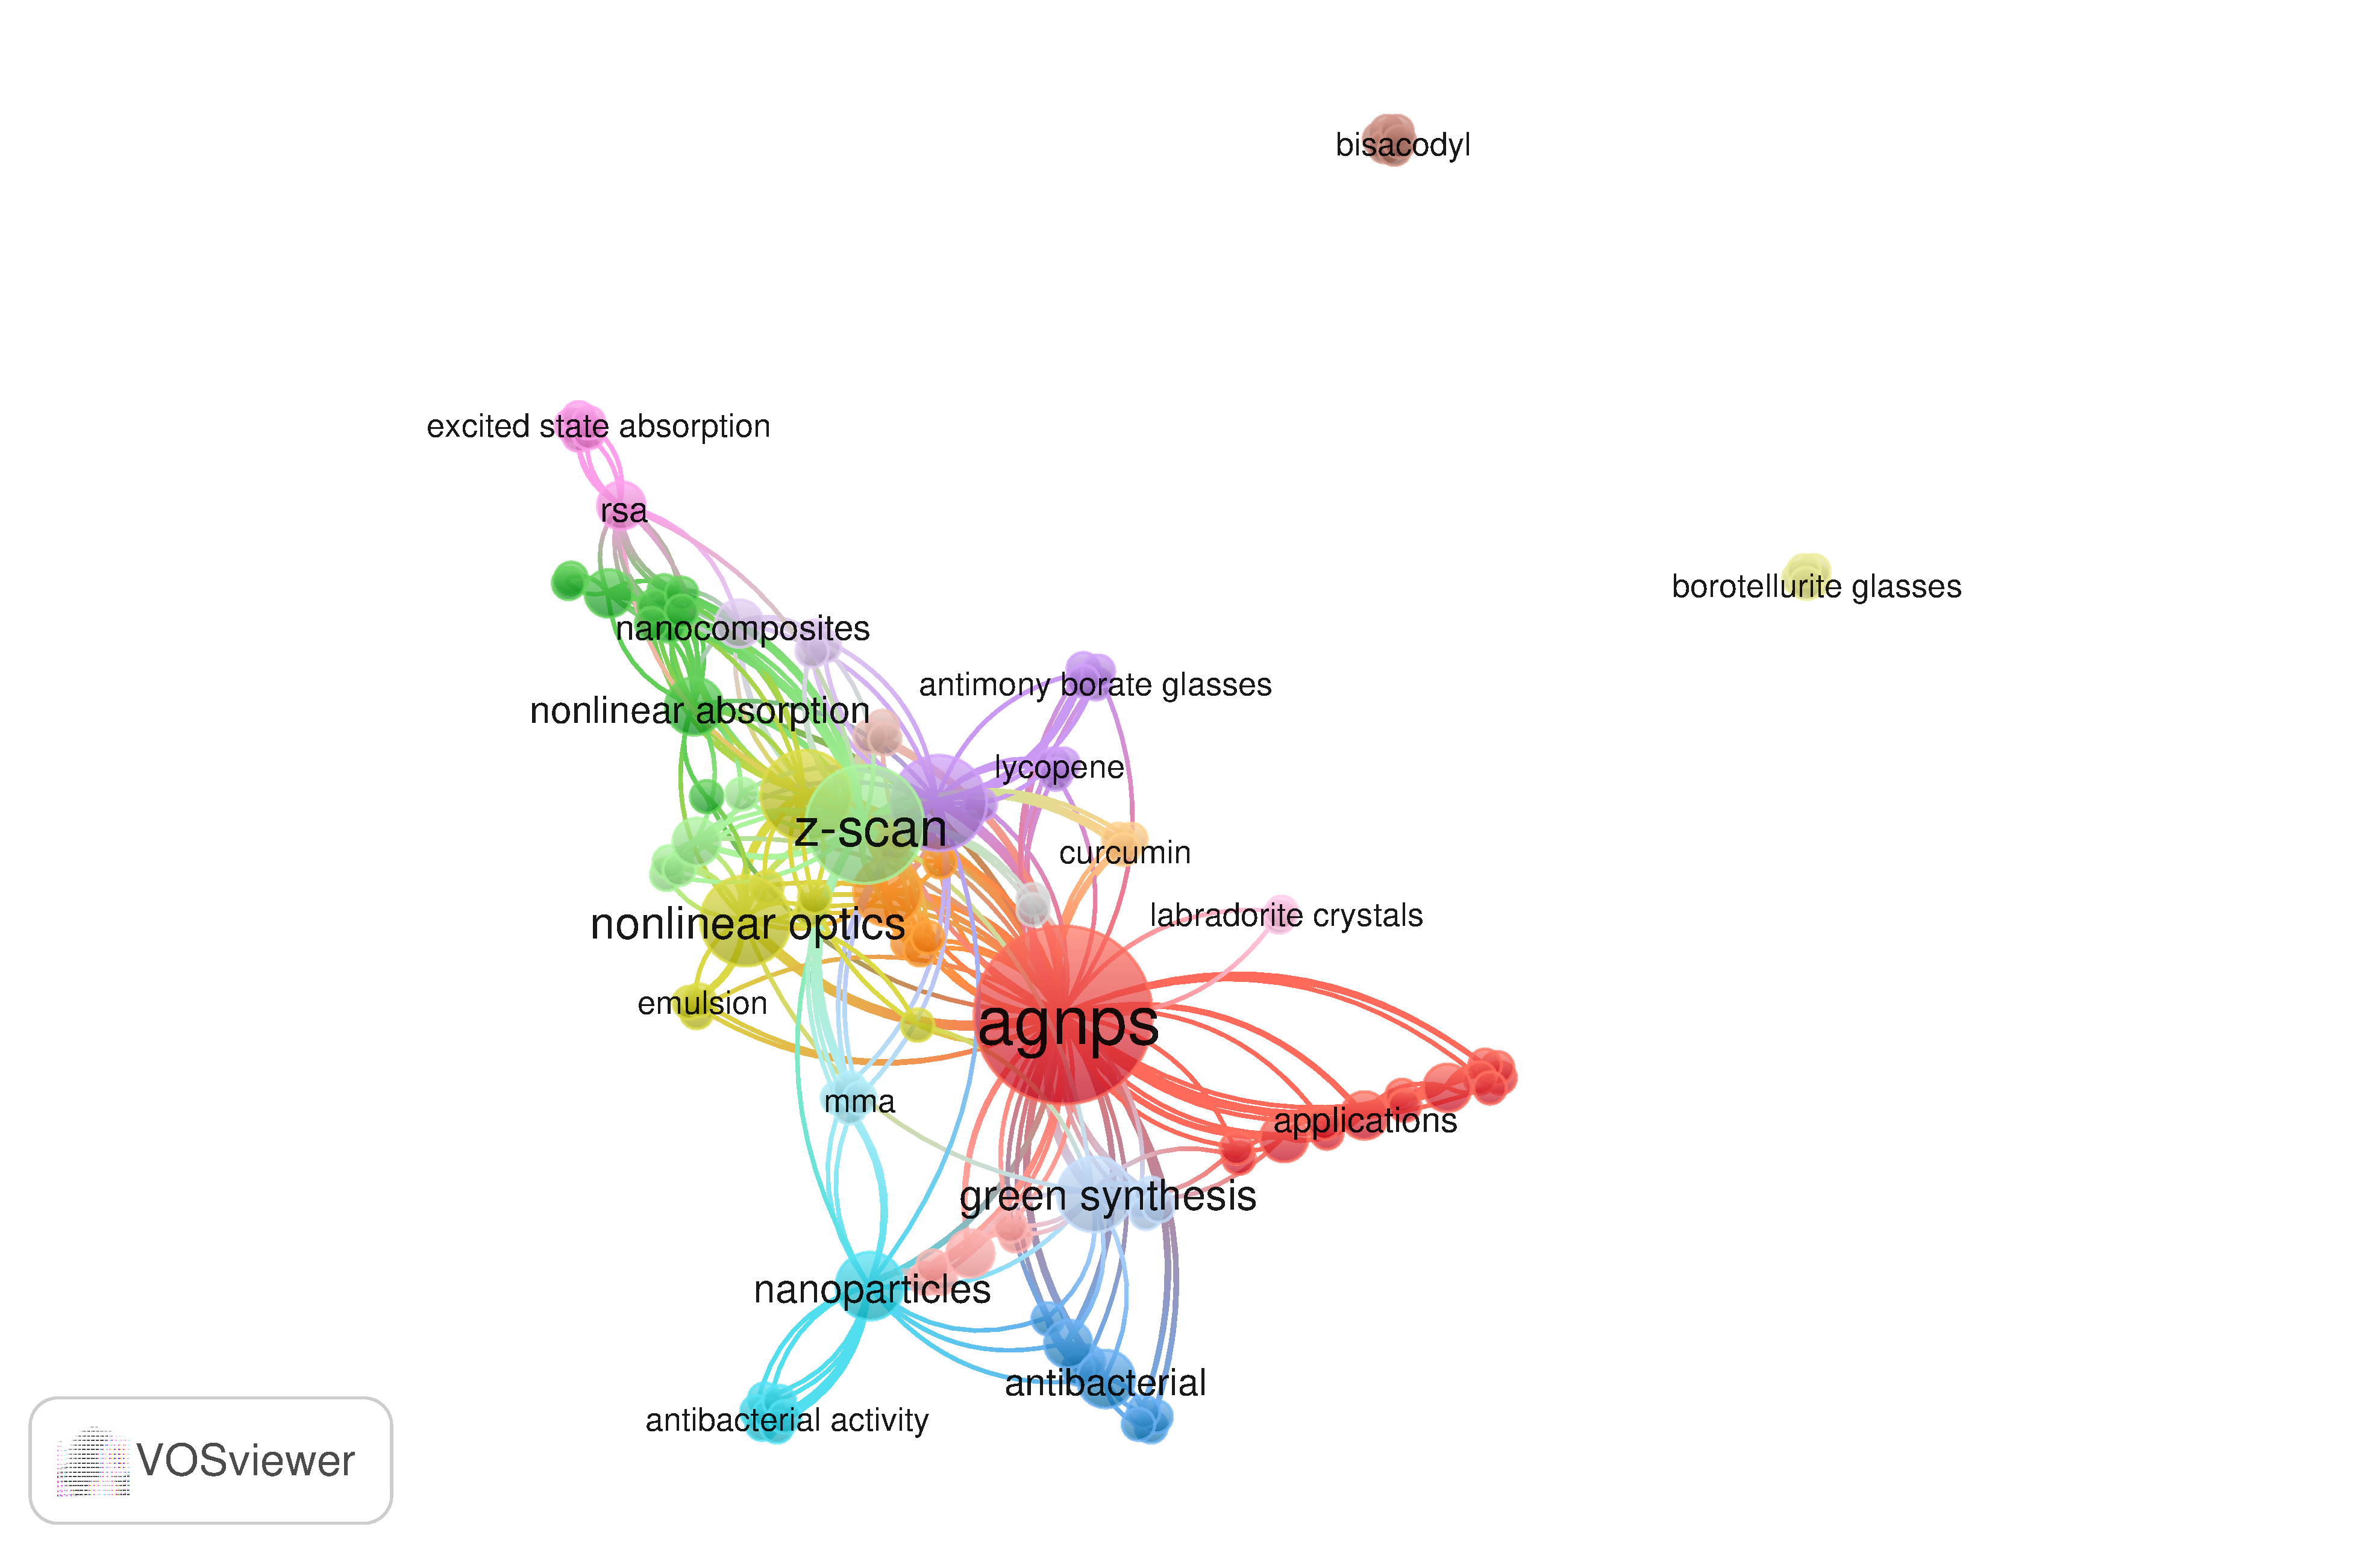
\includegraphics[width=0.8\textwidth]{./key-word-map.pdf}
	\caption{Mapa de coocurrencia de palabras clave de la literatura
	seleccionada sobre AgNPs.}
	\label{fig:keyword_map}
\end{figure}

La red resultante (Figura \ref{fig:keyword_map}) revela un campo altamente
multidisciplinario, bifurcado entre la caracterización optofísica fundamental y
la ciencia de biomateriales aplicados. Aunque el término específico ``AgNPs''
no se encuentra indexado universalmente, la topología de la red identifica
cuatro agrupaciones temáticas definidas que dictarán el orden de la discusión
subsiguiente.

El primer grupo temático corresponde a la síntesis verde. La literatura
evidencia una transición desde las rutas químicas y físicas tradicionales hacia
métodos biogénicos. Este cambio responde a la necesidad de mitigar la toxicidad
y los costos asociados a los agentes reductores convencionales, priorizando
alternativas sostenibles para la obtención de nanopartículas.

El segundo grupo se centra en la caracterización óptica y la física
fundamental. Los términos predominantes incluyen la técnica de escaneo Z, la
óptica no lineal, la absorción saturable y la absorción inversa saturable. Los
datos bibliométricos establecen que el escaneo Z constituye la técnica
experimental estándar para cuantificar la dinámica no lineal de estos
materiales en diversas matrices, fenómenos que serán formalizados
matemáticamente en las siguientes secciones.

Un tercer grupo vincula las propiedades plasmónicas con sus aplicaciones
macroscópicas. La resonancia de plasmón de superficie localizado opera como un
puente conceptual entre la utilidad biomédica, manifestada en la actividad
antibacteriana, y las aplicaciones tecnológicas en fotónica ultrarrápida,
sensores y limitación óptica. Los mecanismos físicos subyacentes que rigen esta
respuesta se detallarán rigurosamente más adelante.

\begin{figure}[htbp!]
	\centering
	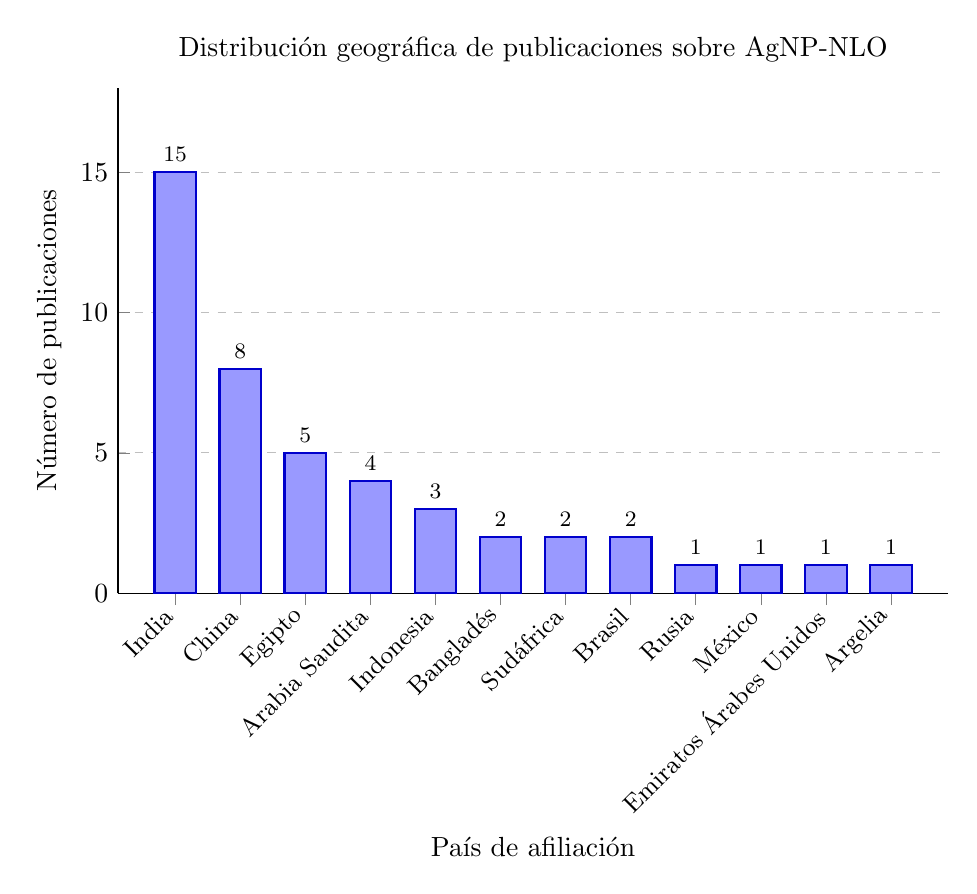
\begin{tikzpicture}
		\begin{axis}[
			ybar,
			bar width=15pt,
			width=\textwidth,
			height=8cm,
			ylabel={Número de publicaciones},
			xlabel={País de afiliación},
			symbolic x coords={India, China, Egipto, Arabia Saudita, Indonesia,
				Bangladés, Sudáfrica, Brasil, Rusia, México,
			Emiratos Árabes Unidos, Argelia},
			xtick=data,
			xticklabel style={rotate=45, anchor=east, font=\small},
			nodes near coords,
			nodes near coords align={vertical},
			nodes near coords style={font=\footnotesize},
			ymin=0,
			ymax=18,
			enlarge x limits=0.08,
			title={Distribución geográfica de publicaciones sobre AgNP-NLO},
			axis lines*=left,
			ymajorgrids=true,
			grid style=dashed,
			]

			\addplot[fill=blue!40, draw=blue!80!black, thick] coordinates {
				(India, 15)
				(China, 8)
				(Egipto, 5)
				(Arabia Saudita, 4)
				(Indonesia, 3)
				(Bangladés, 2)
				(Sudáfrica, 2)
				(Brasil, 2)
				(Rusia, 1)
				(México, 1)
				(Emiratos Árabes Unidos, 1)
				(Argelia, 1)
			};

		\end{axis}
	\end{tikzpicture}
	\caption{Distribución bibliométrica de la producción científica según el
		país de afiliación institucional, destacando las contribuciones
		predominantes de India, China y Egipto en la síntesis y caracterización
	óptica no lineal de AgNPs.}
	\label{fig:country_distribution}
\end{figure}

Finalmente, el análisis de las afiliaciones institucionales, ilustrado en la
Figura \ref{fig:country_distribution}, muestra un esfuerzo investigativo con
una concentración predominante en el Sur Global. La producción científica está
liderada significativamente por India con 15 publicaciones, seguida por China
con 8 y Egipto con 5. Estas naciones encabezan la investigación experimental
sobre vidrios dopados y nanocompuestos, complementadas por contribuciones
sostenidas de Arabia Saudita (4 trabajos), Indonesia (3), y participaciones
de naciones como Bangladés, Sudáfrica y Brasil (2 trabajos cada una).
Esta métrica confirma que el desarrollo de nanomateriales optoelectrónicos
sostenibles y escalables es una prioridad de investigación global.

\subsection{Síntesis biogénica}

La transición de la síntesis química convencional a la biogénica representa un
cambio fundamental en la fabricación de nanomateriales. Desde la fisicoquímica,
este enfoque ascendente está gobernado por la termodinámica de
reducción-oxidación. Los métodos tradicionales emplean agentes reductores
tóxicos para donar electrones, reduciendo los iones argénticos ($\ce{Ag^+}$) a plata
de valencia cero ($\ce{Ag^0}$), seguido de nucleación y crecimiento
\cite{hosnyComprehensiveReviewSilver2025, lasmiSilverNanoparticlesAgNPs2025}.

La síntesis biogénica emplea extractos naturales como sistemas de reacción,
donde los fitoquímicos actúan simultáneamente como agentes reductores y
pasivantes \cite{thomasPlantbasedSynthesisCharacterization2024,
rupanshiBiogenicSilverNanoparticles2025}. Esta mediación biológica minimiza
la energía de activación del proceso termodinámico, omitiendo el uso de
precursores tóxicos y suprimiendo la aglomeración incontrolada
\cite{nagimeMoringaOleiferaPlethora2024}. Físicamente, la estabilización
es crítica: la corona biomolecular conformada por polímeros naturales, como
las redes basadas en quitosano \cite{voChitosanbasedStabilizersAqueous2025},
altera la permitividad dieléctrica local. Esta condición de frontera dicta la
frecuencia de la resonancia de plasmón de superficie localizado, el parámetro
fundamental para las aplicaciones ópticas
\cite{satiSilverNanoparticlesAgNPs2025}. En consecuencia, la evolución
estructural y la densidad de esta capa pasivante determinan la topología del
campo electromagnético local, correlacionándose con una mejora sustancial en
la susceptibilidad óptica \cite{elhendawiEnhancementStructureLinear2025}.
La cuantificación rigurosa de este fenómeno no lineal mediante escaneo Z
exige una caracterización morfológica precisa, pues las secciones eficaces
de absorción dependen estrictamente de la arquitectura del recubrimiento
\cite{al-jumailyCharacterizationNonlinearOptical2025,
kocSilverNanoparticlesAgNPs2026}.

La relevancia biológica de estas nanoestructuras emana de su citotoxicidad,
una propiedad macroscópica dictada por su relación área-volumen y su estado
de superficie. La biofísica de esta actividad antibacteriana depende de
interacciones electrostáticas fundamentales. Los agentes pasivantes
biogénicos confieren una densidad de carga específica a la nanopartícula.
Al aproximarse a las paredes celulares bacterianas, que exhiben una
distribución espacial de carga electronegativa, el acoplamiento mediado por
la interacción de Coulomb determina la probabilidad de adhesión a la membrana
y su subsecuente translocación \cite{hosnyComprehensiveReviewSilver2025,
kannaiahAntibacterialCytotoxicEffect2026}.

Una vez adheridas, los mecanismos físicos de muerte celular proceden a través
de dos vías principales. Primero, la disolución oxidativa impulsada
termodinámicamente libera iones $\ce{Ag^+}$ que se enlazan a los grupos tiol de las
proteínas celulares, interrumpiendo la cadena respiratoria. Segundo, la
superficie plasmónica y catalítica induce la generación de especies reactivas
de oxígeno. Este estrés oxidativo localizado daña físicamente las
macromoléculas, induciendo la peroxidación lipídica y la escisión de las
cadenas de ácido desoxirribonucleico
\cite{thomasPlantbasedSynthesisCharacterization2024}.

Aunque la síntesis biogénica elimina los precursores químicos agresivos,
introduce el paradigma de la toxicología verde. Es erróneo asumir que los
nanomateriales biogénicos son intrínsecamente inocuos, pues la toxicidad de las
AgNPs es dependiente de la dosis y varía significativamente entre modelos
biológicos \cite{nogaToxicologicalAspectsSafety2023}.

Desde la física ambiental, la alta estabilidad conferida por la pasivación
biogénica implica que estas nanopartículas pueden persistir en los ecosistemas.
Las tasas de transporte, agregación y lixiviación iónica en matrices
ambientales constituyen una preocupación crítica. Comprender su estabilidad
termodinámica y perfiles de degradación en dieléctricos ambientales complejos
es imperativo para prevenir la bioacumulación
\cite{thomasPlantbasedSynthesisCharacterization2024,
nogaToxicologicalAspectsSafety2023}.

A pesar del crecimiento en la literatura, persisten vacíos fundamentales en la
física de los nanomateriales verdes. Las interacciones mecánico-cuánticas y
termodinámicas entre los extractos heterogéneos y las facetas cristalinas en
crecimiento son insuficientemente comprendidas. En consecuencia, el control
morfológico exacto permanece como un desafío. Dado que los umbrales de
limitación óptica y las propiedades no lineales son altamente sensibles a la
anisotropía, esto obstaculiza su implementación en fotónica avanzada
\cite{satiSilverNanoparticlesAgNPs2025}.

Asimismo, la variabilidad bioquímica de los extractos vegetales, dependiente de
factores geográficos y estacionales, impide la reproducibilidad de las
cinéticas de reducción \cite{hosnyComprehensiveReviewSilver2025}. Finalmente,
la estructura física precisa de la biocorona y su influencia en la absorción de
estados excitados durante la irradiación láser de alta intensidad requieren
sondeos físicos avanzados, como espectroscopia de absorción transitoria, los
cuales se encuentran ausentes en la literatura actual de biomateriales.

\subsection{Óptica no lineal en AgNPs}

Las propiedades ópticas no lineales de las nanopartículas de plata (AgNPs) las
posicionan a la vanguardia de la nanofotónica moderna. Desde la electrodinámica
fundamental, cuando un medio es sometido a un campo electromagnético intenso, la
polarización macroscópica $P$ inducida pierde su linealidad respecto al campo
eléctrico $E$, describiéndose mediante la expansión en serie de potencias
$$P=\varepsilon_0(\chi^{(1)}E+\chi^{(2)}E^2+\chi^{(3)}E^3+\dots)$$
donde $\chi^{(3)}$ es la susceptibilidad óptica no lineal de tercer orden. En
las AgNPs, los efectos dominantes derivan de las partes real e imaginaria de
$\chi^{(3)}$, manifestándose como refracción no lineal (efecto Kerr óptico,
caracterizado por el índice $n_2$) y absorción no lineal (caracterizada por el
coeficiente $\beta$) \cite{qayyumNonlinearOpticalProperties2025,
zhouSituFormationSilver2024}.
El origen físico de esta susceptibilidad magnificada reside en la resonancia de
plasmón de superficie localizado. La coincidencia entre la frecuencia del láser
incidente y la oscilación colectiva de los electrones de conducción genera un
incremento masivo del campo electromagnético local. Esta amplificación de las
interacciones luz-materia produce valores de $\chi^{(3)}$ que superan por varios
órdenes de magnitud a los de la plata volumétrica o matrices dieléctricas
estándar \cite{tchindangounouSurfacePlasmonEnhanced2025,
mohamedExcitationWavelengthColloids2022}.

Para la cuantificación experimental de estos parámetros, la técnica de escaneo
Z se establece como el marco de referencia. En la configuración de apertura
abierta, se captura la transmitancia dependiente de la intensidad. Dos
mecanismos fundamentales dictan esta dinámica. A intensidades moderadas,
prevalece la absorción saturable, originada por el blanqueamiento plasmónico
del estado fundamental. El alto flujo de fotones agota los electrones más
rápido de lo que pueden relajarse, induciendo transparencia transitoria
\cite{gonzalez-campuzanoSaturableAbsorptionNegative2023}.
Al superar un umbral de intensidad específico,
emerge la absorción inversa saturable, gobernada por la absorción de dos
fotones o la absorción de estados excitados. Los electrones promovidos
absorben secuencialmente fotones adicionales hacia estados superiores, dado
que la sección eficaz del estado excitado supera la del estado fundamental
\cite{mousaviIntrinsicOpticalBistability2025}.
Estudios de alta resolución revelan transformaciones
dinámicas complejas, como la doble transición de absorción saturable a
inversa y nuevamente a saturable, dependiendo de la fluencia láser y del
poblamiento total de los estados excitados
\cite{jiangDoubleTransformationNonlinear2022, jiangSizeEffectNonlinear2022}.

La capacidad de sintonizar la susceptibilidad $\chi^{(3)}$ ha catalizado el
desarrollo de tecnologías fotónicas emergentes. La manifestación macroscópica
más relevante de la absorción inversa saturable es la limitación óptica, un
mecanismo pasivo indispensable para proteger sensores optoelectrónicos contra
radiación láser de alta fluencia. La literatura prioriza la minimización del
umbral de limitación mediante la conjugación de AgNPs con óxido de grafeno,
colorantes y moléculas específicas como el indol-7-carboxaldehído
\cite{lakheraEnhancementOpticalLimiting2025, fathimaPlasmonEnhancedLinear2021,
salahBoostingNonlinearOptical2023,
lakheraIndole7carboxaldehydeFunctionalizedSilver2025}. Estas arquitecturas
híbridas metal-orgánicas, sintetizadas incluso mediante rutas químicas a baja
temperatura, propician una transferencia de carga sinérgica que amplifica la
absorción de estados excitados y maximiza la capacidad de atenuación no lineal
\cite{lakheraLowtemperatureChemicalSynthesis2025}.

Para evadir las inestabilidades termodinámicas de los coloides líquidos bajo
campos de radiación intensos, el confinamiento de las AgNPs en matrices de
estado sólido, como vidrios de borotelurato y redes poliméricas, se establece
como una directriz fundamental \cite{ganjiNonlinearOpticalStructural2025,
al-hadeethiNanosecondNonlinearOptical2022, zhouSituFormationSilver2024}.
La selección de precursores, como \ce{AgNO3} o \ce{AgCl}, modula la
permitividad dieléctrica del medio continuo, permitiendo una sintonización
espectral precisa de la polarización electromagnética. Asimismo, la pasivación
mediante heteroestructuras núcleo-coraza tipo \ce{Ag{@}SiO2} o sistemas de
emulsión inhibe la degradación superficial, preservando la susceptibilidad no
lineal \cite{jagannathanPrecursorBasedTuning2021,
abhiramComparativeStudyAuAg2021,
adampourEmulsionstabilizedSilverNanoparticles2025,
chevychelovaNonlinearOpticalProperties2021}. La incrustación en películas
poliméricas de Ag/PMMA exhibe una absorción no lineal dependiente de la
densidad y dinámicas de autoenfoque \cite{abbasNonlinearOpticalProperties2022},
lo cual también optimiza la estabilidad termodinámica para aplicaciones
biomédicas de liberación controlada \cite{chaionSilverNanoparticleBased2025}.

La interacción del campo electromagnético local se amplifica al integrar las
AgNPs con materiales bidimensionales y semiconductores. En heteroestructuras de
rGO/\ce{MnO2} decoradas con plata, el acoplamiento de las excitaciones
plasmónicas con los estados de banda intermedia incrementa masivamente las
secciones eficaces de absorción no lineal
\cite{dhanushaMidgapStatesMediated2025}. De manera análoga, la interfaz entre
AgNPs y nanoláminas de MXeno (\ce{Ti3C2T_x}) fomenta una transferencia de carga
ultrarrápida, habilitando el diseño de limitadores ópticos de alta eficiencia
\cite{yanEnhancedOpticalNonlinearity2021}. En marcos semiconductor-metal, como
las películas de Ag/CdS, la superposición de la resonancia plasmónica con la
estructura de bandas del semiconductor permite un control determinista sobre la
respuesta óptica \cite{yuStudyNonlinearOptical2026}.

En el dominio teórico, el control riguroso de las tasas de acoplamiento y
transición entre los regímenes de absorción saturable e inversa facilita la
emergencia de biestabilidad óptica intrínseca. Este comportamiento de
histéresis en la transmisión fundamenta la arquitectura de compuertas lógicas
puramente ópticas y establece la base física para dispositivos de conmutación
fotónica ultrarrápida \cite{mousaviIntrinsicOpticalBistability2025}.

A pesar de la observación macroscópica detallada de estas no linealidades,
persisten vacíos profundos en el aislamiento de los mecanismos físicos
fundamentales. Un desafío crítico en el escaneo Z de apertura cerrada es la
discriminación del efecto de lente térmica respecto a la no linealidad
electrónica pura. La termalización de la energía absorbida induce gradientes
de índice de refracción que enmascaran el efecto Kerr instantáneo,
particularmente bajo irradiación con láseres de alta tasa de repetición
\cite{qayyumNonlinearOpticalProperties2025}.
Adicionalmente, la fotodegradación bajo alta fluencia
representa un obstáculo no resuelto. Las AgNPs desprotegidas sometidas a
campos láser intensos sufren fusión o remodelación geométrica durante la
irradiación, alterando dinámicamente su respuesta en el tiempo de medición
\cite{chevychelovaNonlinearOpticalProperties2021,
gonzalez-campuzanoSaturableAbsorptionNegative2023}.
Por último, la integración de metodologías de síntesis verde introduce una alta
polidispersidad morfológica.  Dado que las secciones eficaces de dispersión y el
confinamiento cuántico son hipersensibles al radio y la geometría, esta
heterogeneidad difumina los umbrales de inicio de los procesos de absorción no
lineal, dificultando la formulación de modelos teóricos cuantitativos unificados
para biocompuestos fotónicos de nueva generación
\cite{josephBiogenicSilverNanoparticles2026,
tchindangounouCorrectionSurfacePlasmon2025}.

\subsection{Resonancia de plasmón de superficie localizado}

Las propiedades ópticas, no lineales y catalíticas excepcionales de las
nanopartículas de plata (AgNPs) tienen su origen fundamental en su
comportamiento plasmónico. Cuando una onda electromagnética interactúa con una
nanopartícula metálica cuyas dimensiones son significativamente menores que la
longitud de onda ($d\ll\lambda$), el campo eléctrico oscilante desplaza los
electrones de la banda de conducción respecto al núcleo iónico con carga
positiva. Este desplazamiento induce una interacción de Coulomb restauradora que
resulta en una oscilación coherente y colectiva de la nube electrónica,
fenómeno denominado resonancia de plasmón de superficie localizado
\cite{thomasPlantbasedSynthesisCharacterization2024,
qayyumNonlinearOpticalProperties2025}.

Desde la perspectiva de la física del estado sólido, la condición de
resonancia para una nanopartícula esférica se deriva de la aproximación
cuasiestática de la teoría de Mie.
En el sistema cegesimal (CGS), la polarizabilidad $\alpha$ de la nanopartícula
está dada por la relación de Clausius-Mossotti
\begin{equation}
	\alpha=4\pi
	R^3\frac{\varepsilon_m(\omega)-\varepsilon_d}{\varepsilon_m(\omega)+2\varepsilon_d}
\end{equation}
donde $R$ es el radio de la partícula,
$\varepsilon_m(\omega)=\varepsilon_1(\omega)+i\varepsilon_2(\omega)$ es la
función dieléctrica compleja dependiente de la frecuencia del metal, y
$\varepsilon_d$ es la constante dieléctrica del medio circundante. La
resonancia ocurre cuando el denominador tiende a cero, conocida como la
condición de Fröhlich, $\varepsilon_1(\omega)=-2\varepsilon_d$. Dado que la
plata posee una componente dieléctrica imaginaria ($\varepsilon_2$)
intrínsecamente baja en el espectro visible en comparación con el oro o el
cobre, las AgNPs exhiben picos de resonancia excepcionalmente agudos e
intensos, constituyéndose como los resonadores plasmónicos más eficientes en
longitudes de onda visibles \cite{kelaniComparingSilverGold2024,
satiSilverNanoparticlesAgNPs2025}.

La excitación del plasmón de superficie conduce a secciones eficaces masivas
de absorción y dispersión en el campo lejano, junto con un confinamiento
intenso de la energía electromagnética en el campo cercano. Este confinamiento
es el mecanismo subyacente de la dispersión Raman amplificada por superficie.
Al adsorber un analito sobre la superficie plasmónica, la señal Raman,
característicamente débil, se amplifica por un factor proporcional a $|E|^4$,
donde $E$ es el campo eléctrico local. La integración de AgNPs en matrices de
carbono genera puntos calientes plasmónicos que permiten la detección de
moléculas a nivel de ultratrazas \cite{saadNovelSynthesisStudy2020}.
De manera análoga, aunque las superficies metálicas desnudas suelen extinguir la
fluorescencia mediante transferencias no radiativas, una separación precisa
entre la nanopartícula y el fluoróforo induce fluorescencia amplificada por
metal.
El intenso campo local incrementa la tasa de excitación del fluoróforo, mientras
que el acoplamiento plasmónico eleva la tasa de decaimiento radiativo, un
mecanismo dual que amplifica sinérgicamente la respuesta óptica lineal y no
lineal de colorantes naturales \cite{fathimaPlasmonEnhancedLinear2021}.
Además, como la condición de Fröhlich
depende estrictamente de la permitividad del entorno, cualquier evento de
unión biomolecular en la superficie altera el índice de refracción local,
provocando un corrimiento espectral medible en la longitud de onda de
resonancia. Esta sensibilidad superior, producto de los límites geométricos
agudos de sus secciones eficaces plasmónicas, es explotada en el diseño de
biosensores optofluídicos \cite{kelaniComparingSilverGold2024}.

A pesar de la consolidación de la plasmónica clásica, la integración de AgNPs en
arquitecturas fotónicas avanzadas enfrenta limitaciones teóricas y materiales.
La electrodinámica clásica predice una divergencia en el campo electromagnético
local cuando la distancia interpartícula tiende a cero. No obstante, en brechas
subnanométricas, el efecto túnel mecánico-cuántico de los electrones atenúa
esta divergencia, suprimiendo el acoplamiento plasmónico. La formulación de
modelos teóricos que incorporen correcciones cuánticas para estas interacciones
extremas de campo cercano constituye un desafío sustancial. Físicamente, la
superficie de plata exhibe una alta reactividad ambiental, originando óxidos
como el \ce{Ag2O} y sulfuros. Esta alteración en las condiciones de frontera
dieléctricas incrementa la componente imaginaria de la permitividad, induciendo
un amortiguamiento plasmónico severo y ensanchamiento espectral. La pasivación
mediante heteroestructuras núcleo-coraza tipo \ce{Ag{@}SiO2} o sistemas
bimetálicos \ce{Ag{@}Au} mitiga esta degradación, aunque la barrera de potencial
introducida por la coraza atenúa las interacciones de campo cercano con el
entorno, exigiendo un mapeo experimental más riguroso
\cite{chevychelovaNonlinearOpticalProperties2021,
silva-silvaBiosynthesisAgAuBimetallic2023}.

Finalmente, el desarrollo de conmutadores ópticos no lineales y biosensores
requiere una respuesta colectiva homogénea. La polidispersidad dimensional y la
agregación inherentes a las metodologías sintéticas actuales provocan un
ensanchamiento inhomogéneo de la línea de resonancia. Esta variabilidad
difumina los límites de detección de molécula única y obstaculiza la
extrapolación teórica desde la dinámica de absorción de dispersores individuales
\cite{elimLargeNonlinearAbsorption2021} hacia la ingeniería de arreglos
macroscópicos escalables. En conjunto, la convergencia entre el confinamiento
de las excitaciones plasmónicas y el control determinista de su síntesis
expande las fronteras de investigación en AgNPs. Esta intersección proyecta el
estudio desde la electrodinámica fundamental hacia la consolidación de
aplicaciones optoelectrónicas y biomédicas integrales
\cite{chaoOpticalPropertiesApplications2024}.
